\begin{multicols}{3}[\section {D-Netz}]

\rhead{Autor:Tizian Kurkamp}
\lfoot{Letzte Bearbeitung: 15.04.2016}

\newrefsegment

\begin{boxedminipage}{\linewidth}
\begin{tabular}{p{2,1 cm}p{2.7 cm}}
\textbf{Steckbrief}& \\
\end{tabular}
\begin{tabular}{p{2,1 cm}|p{2.7 cm}}
      Einsatz seit & 1992\\
      \hline
      Frequenz"-bereich  & \SI{890} - \SI{960}{\mega\hertz}\\
      \hline
      Modulationsart & GMSK\\
      \hline
      Bandbreite eines Kanals & \SI{200}{\kilo\hertz}\\
      \hline
      Sendeleistung der Basisstation & <\SI{50}{\watt}\\
      \hline
      Sendeleistung im Endgerät & Handy:  \SI{2}{\watt}, "Auto bis \SI{14}{\watt}\\
\end{tabular}
\end{boxedminipage}
\par
%Source http://www.fh-bingen.de/fileadmin/user_upload/Lehrende/Kilsch_Dieter/internet/projekte/TedoSchStiUnits.pdf -> Seite 9 findet ihr alle verwendbaren Einheiten, wie:
%\SI{Zahl}{\mega\hertz} oder \SI{Zahl}{\mili\metre}
%Ich weiß ehrlich gesagt nicht welche Einheiten ihr im Text genau braucht, aber in dem Dokument und mit obigen Beispiel sollte es umsetzbar ein.

\subsection*{Überblick}


Das D-Netz ist ein zellulares Mobilfunknetz nach dem GSM-Standard. Die Namensgebung durch den Buchstaben D erfolgt in Fortsetzung der bisherigen Buchstabenbezeichnung für die Funknetze.
Das D-Netz ist digitalisiert, sowohl was die Wählvermittlung (Signalling) anbelangt als auch für Übertragung von Daten und Sprache. Letztere werden quantisiert, digitalisiert und pulscodemoduliert, wodurch sie störungsarm und regenerierbar sind und somit auch unter schwierigen Bedingungen übertragen werden können. Besonderes Kennzeichen dieses Zellularnetzes ist das automatische Handover und das automatische Auffinden von Teilnehmern, deren Standort nicht bekannt ist, selbst dann, wenn derzeit kein Gespräch geführt wird und keine Datenverbindung besteht.

Unter dem Namen D-Netz (oder auch DNetz) werden gleich zwei Netze zusammengefasst. Sowohl die Telekom (D1) als auch Vodafone nutzen D-Netz Frequenzen um ihre Mobilfunk-Dienste abzuwickeln. Das D-Netz stand ursprünglich für ein digitales Netz im GSM-900-Frequenzbereich und wurde dann später durch das E-Netz (genutzt von E-Plus und O2) erweitert. Die Namen D1-Netz (für das Netz der Telekom bzw. T-Mobile) und D2-Netz (für das Netz von Vodafone) leiten sich noch aus der ursprünglichen Aufteilung ab.
Mittlerweile gibt es mit UMTS-Netze und LTE Netzen deutlich mehr Mobilfunk-Netze, die genutzt werden können, die Bezeichnungen haben sich aber mittlerweile so eingebürgert, dass auch ohne die eigentliche Netz-Grundlage viele Nutzer diese Kennungen verwenden.


\subsection*{Technische Erläuterungen}

Die Übertragung findet im 900-MHz-Bereich statt, und zwar in den Teilbereichen 890 MHz bis 915 MHz und 935 MHz bis 960 MHz. Der untere Frequenzbereich wird für die Übertragung vom Mobilfunk-Sender/Empfänger zur Basisstation benutzt (Uplink), der obere für die entgegengesetzte Richtung (Downlink). Die Mobilstation wird mit Handy bezeichnet und hat eine Sendeleistung von 0,8 W bis 5 W. Die jeweils 25 MHz breiten Frequenzbereiche, sind in 124 Kanäle unterteilt, von denen jeder 200 kHz breit ist Zur Modulation wird das Gaussian Minimum Shift Keying (= GMSK) verwendet. 

\begin{Figure}
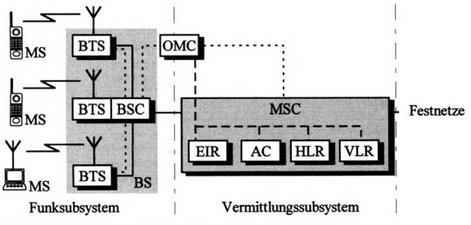
\includegraphics[width=\linewidth]{Kapitel/DNetz/Grafiken/systemaufbau.png}
\captionof{figure}{Systemaufbau des D-Netzes~\cite{vorlage.2}}
\label{fig:vorlage.systemaufbau}
\end{Figure}

Entsprechend der Abbildung \ref{fig:vorlage.systemaufbau} besteht das D-Netz aus der 

\begin{itemize}
	\item Mobilen Station (MS) \\
	Die im Allgemeinen ein Funktelefongerät darstellt. Es kann sich aber prinzipiell um jedes D-Netz-kompatibles Endgerät handeln, 		 	z.B. einen Laptop mit Sende und Empfangseinheit.
	\item Basis Station (BS)
	unterteilt in
		\begin{itemize}
			\item Base Transceiver Station (BTS)
			als reinem Funksende- und Empfangsteil
			\item Base Station Controller (BSC)
			als Steuerungsteil
		\end{itemize}
	\item Funkvermittlung (Mobile Service Switching Center = MSC) mit je einer 
		\begin{itemize}
			\item Besucherdatei (Visitor location Register = VLR)
			\item Heimatdatei (Home Location Register = HLR)
			\item Authentifizierungszentrale (Authentification Center = AC)
			\item Endgerätkennungsdatei (Equipment Identity Register = EIR)
		\end{itemize}
	\item Zentralen Betriebstechnik (Operation and Maintenance Center = OMC)
\end{itemize}






\subsection*{Anbieter}

Für das D-Netz gibt es zwei Betreiber: Die Telekom mit dem D1-Netz und Vodafone mit dem D2-Netz. Da beide Netze nach dem GSM-Standard betrieben werden, gibt es technisch kaum Unterschiede. Damit man die beiden Betreiber an den Rufnummern unterscheiden kann, sind die Netzkennzahlen unterschiedlich.

Anbieter im D1-Netz  (Telekom)

\begin{itemize}
\item chixx
\item congstar
\item Deutsche Telekom
\item freenetmobile
\item ja!mobil
\item Lebara
\item Penny Mobil
\item sparhandy
\item turkcell
\end{itemize}

Anbieter im D2-Netz (Vodafon)

\begin{itemize}
\item 1und1
\item BILDmobil
\item callmobile.de
\item discotel
\item EDEKA Mobil
\item EWE
\item FYVE
\item klarmobil
\item mobilcom debitel
\item otelo
\item Rossmann mobil
\item smartmobil
\item Vodafone
\end{itemize}
(Vgl. ~\cite{vorlage.1})



\end{multicols}
\newpage
\section*{Historische Entwicklung}
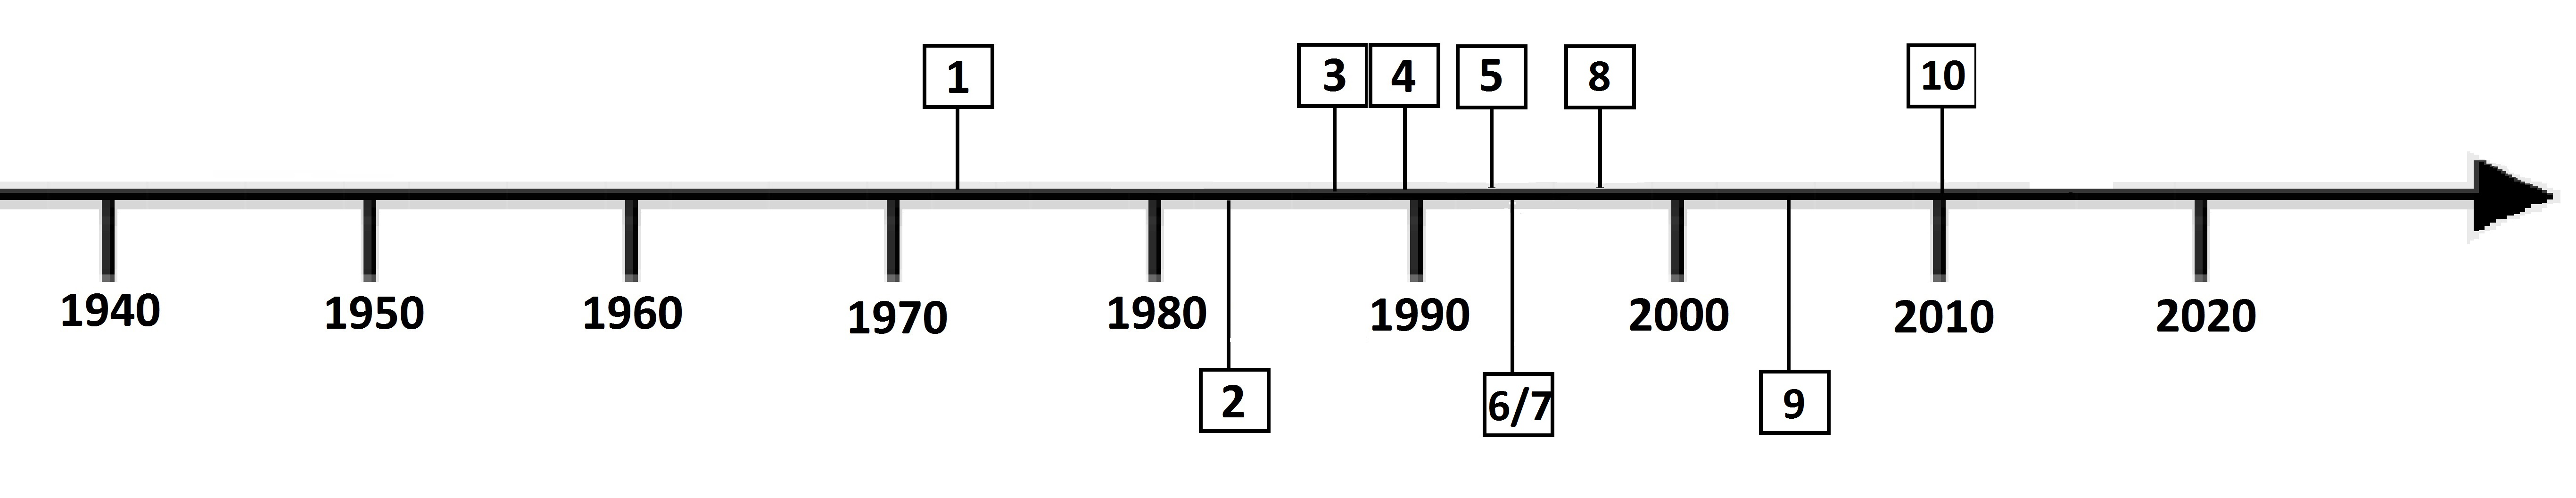
\includegraphics[width=\textwidth]{Kapitel/DNetz/Grafiken/Zeitstrahl}
\par
\noindent
\begin{tabular}{|p{1 cm}|p{3 cm}|p{13.55 cm}|}
	\hline
	Nummer & Datum & Entwicklungsschritte~\cite{vorlage.3}\\
	\hline
	1 & 1972 & Realisierung des B-Netzes\\
	\hline
	2 & 1982 & Gründung der Groupe Speciale Mobile (GSM)\\
	\hline
	3 & 1986 & Einführung des C-Netzes\\
	\hline
	4 & 7. Dezember 1989 & Vergabe einer Lizenz an ein Konsortium unter der Führung des Mannesmann-Konzerns\\
	\hline
	5 & 1. Juli 1992 & Start des Regelbetriebs des D- Netzes\\
	\hline
	6 & April 1993 & ca. 130.000 Netz-Teilnehmer bei der Telekom\\
	\hline
	7 & Ende 1993 & 80ige Abdeckung Deutschlands durch das D2-Netz\\
	\hline
	8 & 1994/95 &  Einführung des E-Plus-Mobilfunknetzes\\
	\hline
	9  & 2004 &  ca. 71 Millionen Mobilfunknutzer und Einführung des UMTS-Netzes\\
	\hline
	10 & 2010 & Einführung des LTE-Mobilfunkstandards\\
	\hline
\end{tabular}
\par
\begin{multicols}{3}

1982 wurde die Groupe Speciale Mobile gegründet, die für Europa ein einheitliches digitales Mobilfunksystem entwickeln sollte. Als sich Ende der 1980er Jahre die praktische Umsetzung des Standards abzeichnete, wurde in Deutschland vom Postminister Christian Schwarz-Schilling entschieden, dass neben der Bundespost auch ein privater Anbieter eine Lizenz für den Betrieb eines Netzes des GSM-Standards erhalten sollte. In dem Ausschreibungsverfahren wurde festgelegt, dass zwischen beiden Betreibern faire Wettbewerbsbedingungen bestehen sollten. Insgesamt zehn Firmen bewarben sich um die Lizenz, die am 7. Dezember 1989 schließlich an ein Konsortium unter Führung des Mannesmann-Konzerns vergeben wurde, das nach Meinung des Lenkungsausschusses Mobilfunk den leistungsfähigsten Bewerber darstellte.
Nach einer einjährigen Versuchsphase wurde der Regelbetrieb am 1. Juli 1992 gestartet. Als unmittelbarer Nachfolger des C-Netzes erhielt das neue Netz die Bezeichnung „D-Netz“.
Das D1-Netz ist das Netz der Deutschen Telekom, während das D2-Netz das Mobilfunknetz der Firma Vodafon bezeichnet, ehemals Mannesmann Mobilfunk. Nach der Einführung des E-Plus-Mobilfunknetzes 1994 setzte ein erheblicher Preisfall bei den Endgeräten, sowie bei der Tarifstruktur ein, sodass die Teilnehmerzahl rapide stieg.(Vgl. ~\cite{vorlage.3} und ~\cite{vorlage.4})

\subsection*{Ausblick}

Als das Handy sich in den 1990er-Jahren in Deutschland etablierte, war Mobilfunk noch etwas Besonderes und die Nutzung von Handys vorwiegend auf das Telefonieren und SMS-Schreiben beschränkt. Auch die Netzabdeckung steckte in Deutschland noch in den Kinderschuhen. Heute gehört das Smartphone mit seinen vielseitigen Funktionen zum Standard des modernen Menschen. Mobil Surfen, Telefonieren, Chatten oder Bilder versenden ist dank moderner Mobilfunknetze problemlos auch unterwegs möglich. Vor allem der neue Standard LTE verspricht Internetgeschwindigkeiten, wie man sie bisher nur von DSL im Heimbereich gewohnt war.
Die vier großen Mobilfunkbetreiber, die Telekom, o2, Vodafone und E-Plus kommen in Deutschland auf eine nahezu vollständige GSM-Netzabdeckung. Somit sollten Sie mit jedem Anbieter fast überall in Deutschland problemlos telefonieren oder eine Kurznachricht versenden können. In Deutschland haben wir also im GSM-Netz eine Netzabdeckung von nahezu 100 Prozent! Allerdings zeigt es sich in der Praxis des Öfteren, dass in manchen Gebieten beim Telefonieren Funklöcher entstehen. Außerdem gibt es noch Unterschiede in der Netzabdeckung mit den verschiedenen Übertragungsarten wie UMTS oder LTE.

Schnelle Übertragungsraten sind theoretisch auch heute schon per LTE Advanced möglich. Die zukünftige Entwicklung der Mobilfunkstandards wird demnach nicht allein von der bereits erreichten Bandbreite, sondern noch viel stärker davon abhängen, wie gut die Netze ausgebaut werden, damit auch das gesamte Leistungsspektrum genutzt werden kann.

Ein wichtiger Motor für den Ausbau der Mobilfunkstandards ist u.a. auch der Mobile Commerce als Teil des E-Commerce. Denn immer mehr Menschen kaufen auch mit ihrem Tablet oder Smartphone im Internet ein. Durch den flächendeckenden Ausbau des LTE-Netzes ist es dann auch möglich, überall und jederzeit in Deutschland online einzukaufen. Auch die Internetnutzung allgemein wird LTE verändern, denn bei voller Netzabdeckung wäre niemand mehr in Deutschland auf einen Festnetzanschluss angewiesen, um schnelles Internet zu nutzen. Vielleicht werden dann in Zukunft auch Festnetzanschlüsse obsolet?

LTE ist zukunftsweisend, der Netzausbau des mobilen Internets wird voraussichtlich den Ausbau des DSL-Netzes in Deutschland übertreffen. Für Bewohner in ländlichen Regionen wäre dies zukünftig eine gute Nachricht, denn sie sind bis dato immer noch vom schnellen Breitbandinternet abgeschnitten.


\printbibliography[segment=11,heading=subbibliography]
\end{multicols}
\newpage